% -*- latex -*-
%%%%%%%%%%%%%%%%%%%%%%%%%%%%%%%%%%%%%%%%%%%%%%%%%%%%%%%%%%%%%%%%
%%%%%%%%%%%%%%%%%%%%%%%%%%%%%%%%%%%%%%%%%%%%%%%%%%%%%%%%%%%%%%%%
%%%%
%%%% This text file is part of the lecture slides for
%%%% `Parallel Computing'
%%%% by Victor Eijkhout, copyright 2012-6
%%%%
%%%% ParLoop-slides.tex : slides about OpenMP's fork-join model
%%%%
%%%%%%%%%%%%%%%%%%%%%%%%%%%%%%%%%%%%%%%%%%%%%%%%%%%%%%%%%%%%%%%%
%%%%%%%%%%%%%%%%%%%%%%%%%%%%%%%%%%%%%%%%%%%%%%%%%%%%%%%%%%%%%%%%

\begin{frame}{Loop parallelism}
  Much of parallelism in scientific computing is in loops:
  \begin{itemize}
  \item Vector updates and inner products
  \item Matrix-vector and matrix-matrix operations
  \item Finite Element meshes
  \item Multigrid
  \end{itemize}
\end{frame}

\begin{frame}[containsverbatim]{Work distribution}
  \begin{itemize}
  \item Suppose loop iterations are independent:
  \item Distribute them over the threads:
  \item Use \indextermtt{omp_get_thread_num} to determine disjoint subsets.
  \item How would you do this specifically?
  \end{itemize}
\end{frame}

\begin{frame}[containsverbatim]{Workshare constructs}
  Here's the two-step parallelization in OpenMP:
  \begin{itemize}
  \item You use the \indextermtt{parallel} directive to create a team of
    threads;
  \item then you use a `workshare' construct to distribute the
    work over the team.
  \item For loops that is the \indextermtt{for} (or \indextermtt{do}) construct.
  \end{itemize}
\end{frame}

\begin{frame}[containsverbatim]{Workshare construct for loops}
C: directive followed by statement or block:
\begin{verbatim}
#pragma omp parallel
{
#pragma omp for
  for (i=0; i<N; i++)
    ... something with i ...
}
\end{verbatim}
Fortran: matching end directive
\begin{verbatim}
!$omp parallel
!$omp do
  do i=1,n
    ... something with i ...
  end do
!$omp end do
!$omp end parallel
\end{verbatim}
\end{frame}

\begin{frame}[containsverbatim]{Stuff inside a parallel region}
\footnotesize
\begin{multicols}{2}  
\begin{verbatim}
#pragma omp parallel
{
  code1();
#pragma omp for
  for (i=1; i<=4*N; i++) {
    code2();
  }
  code3();
}
\end{verbatim}
\columnbreak
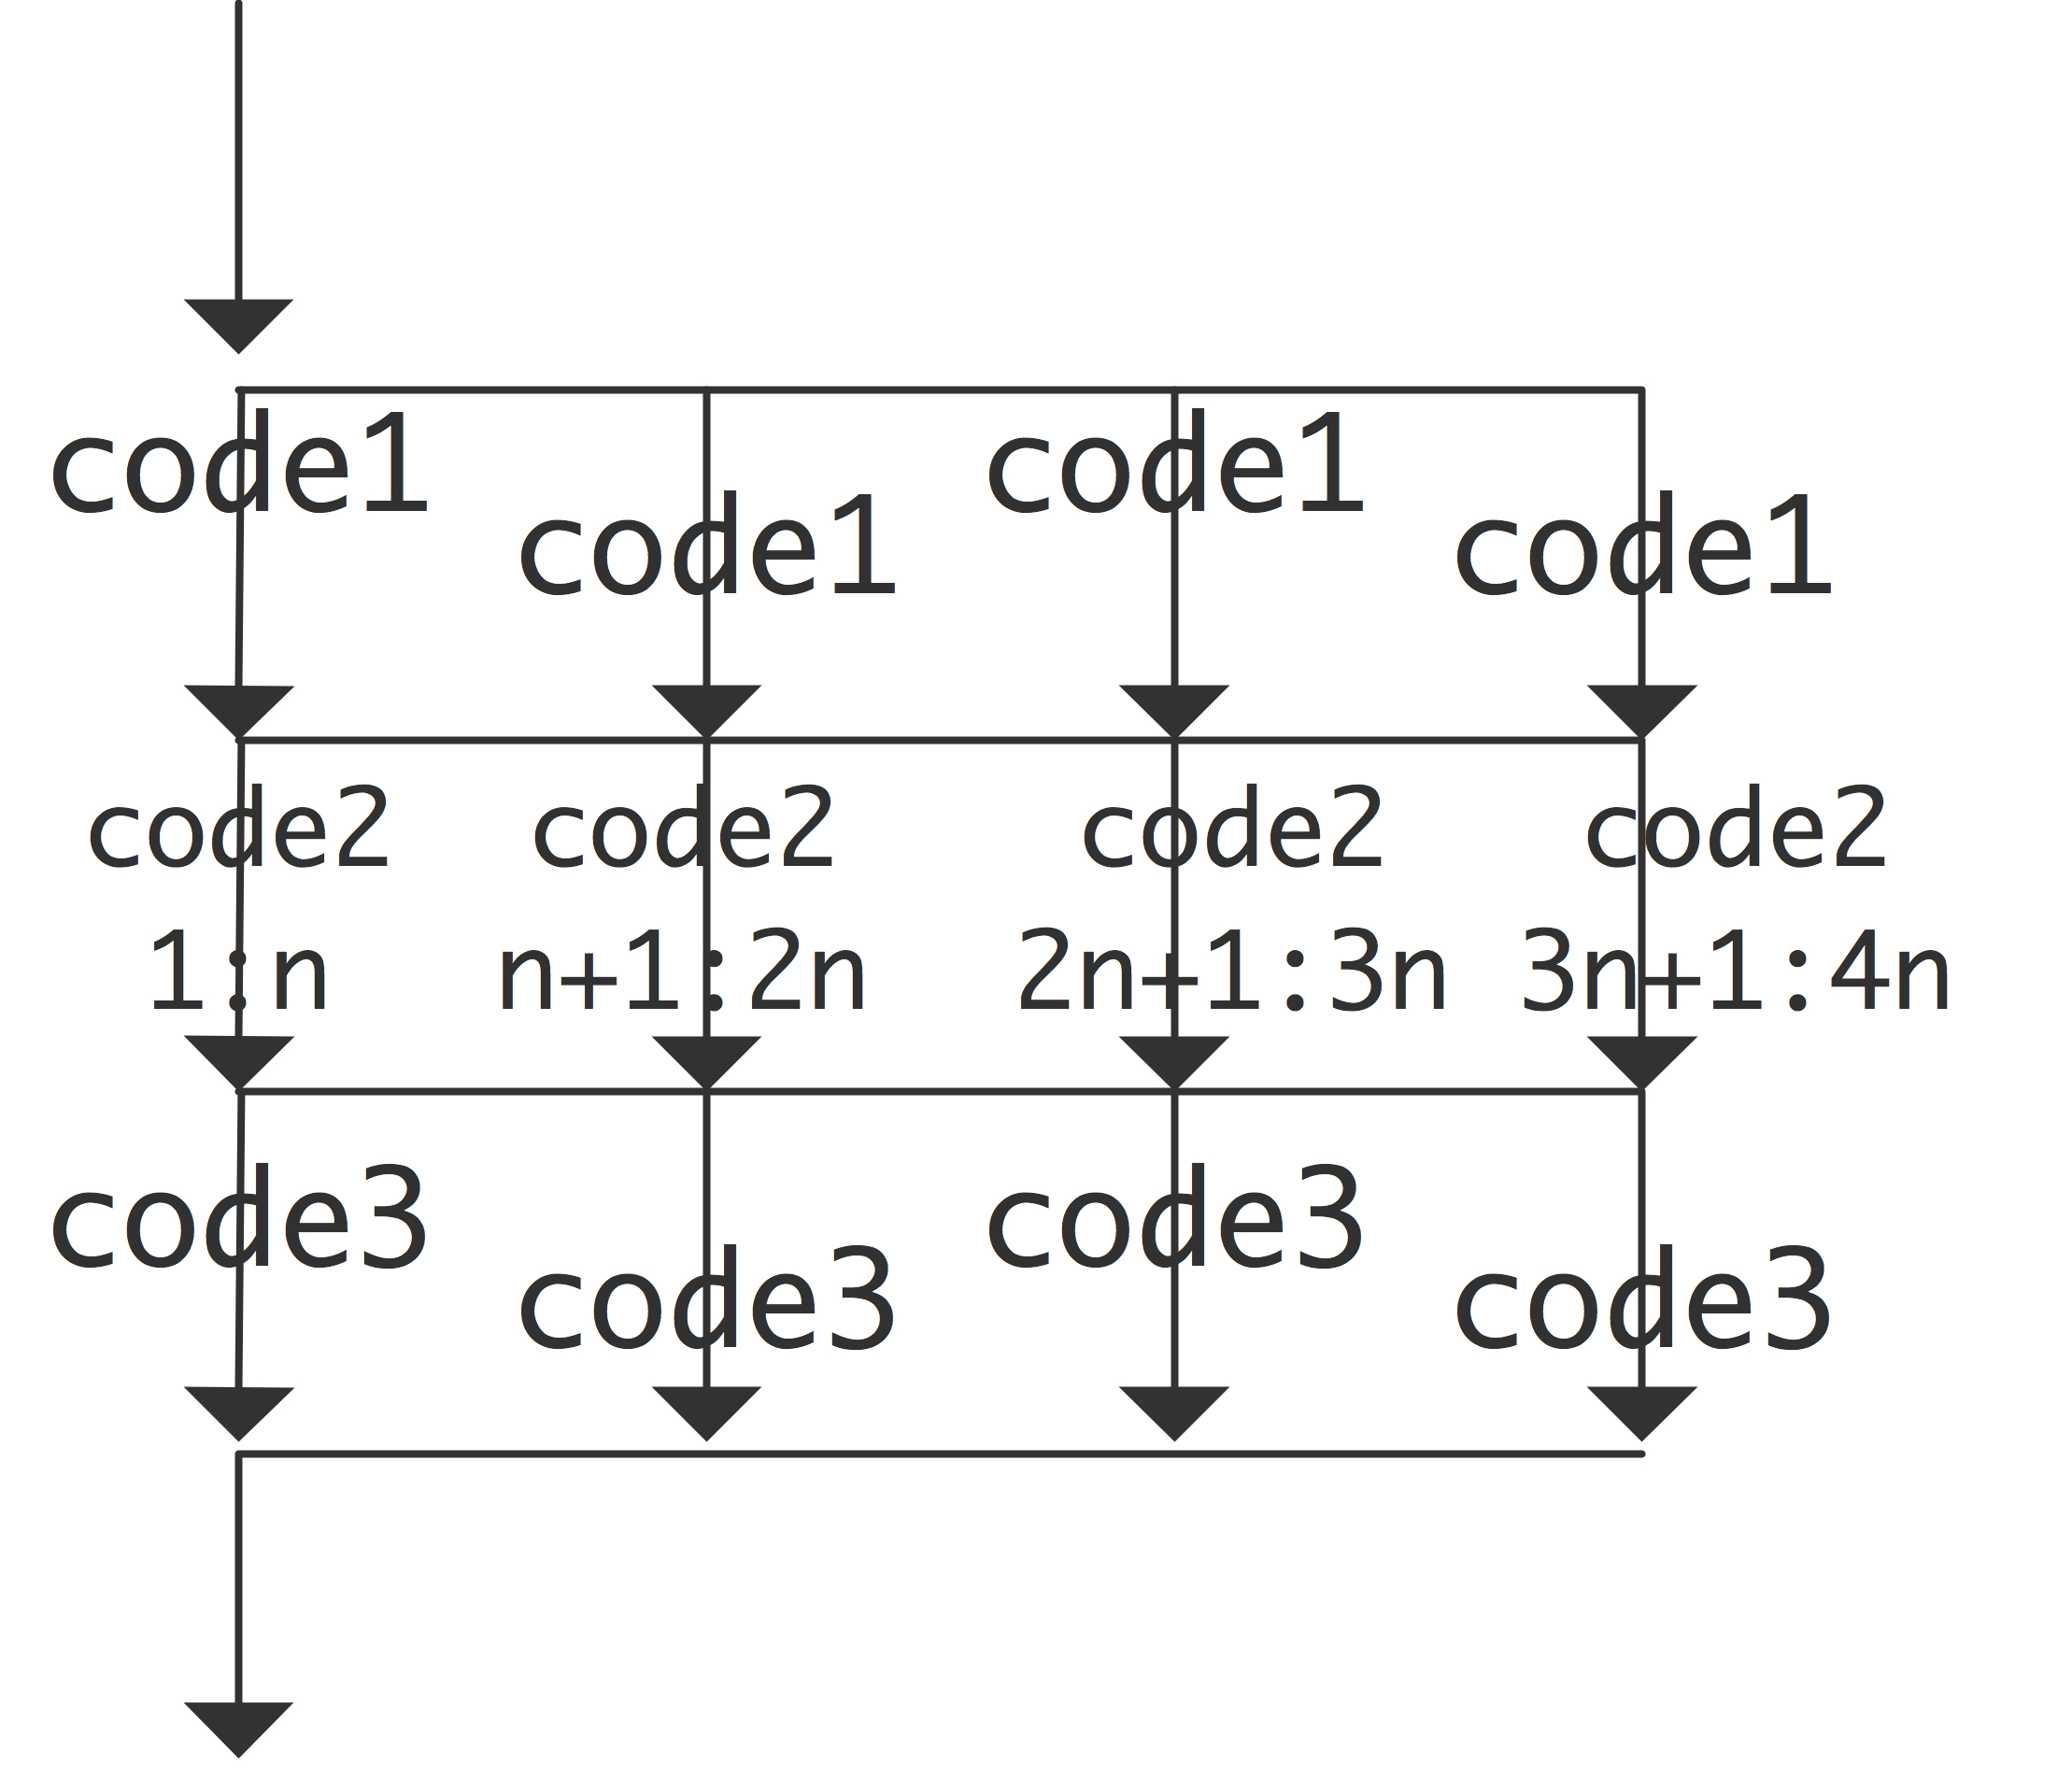
\includegraphics[scale=.07]{parallel-do}
\end{multicols}
\end{frame}

\begin{exerciseframe}[pi]
  \footnotesize
  \input ex:omp-pi
\end{exerciseframe}

\begin{frame}[containsverbatim]{Loop schedules}
  \begin{itemize}
  \item Default: static scheduling of iterations. \\
    Very efficient. Good if all iterations take the same amount of
    time.\\ \texttt{schedule(static)}
  \item Other possibility: dynamic.\\
    Runtime overhead; better if iterations do not take the same amount
    of time.\\
    \texttt{schedule(dynamic)}
  \end{itemize}

  Four threads, 8 tasks of decreasing size\\
  dynamic schedule is better:
  
  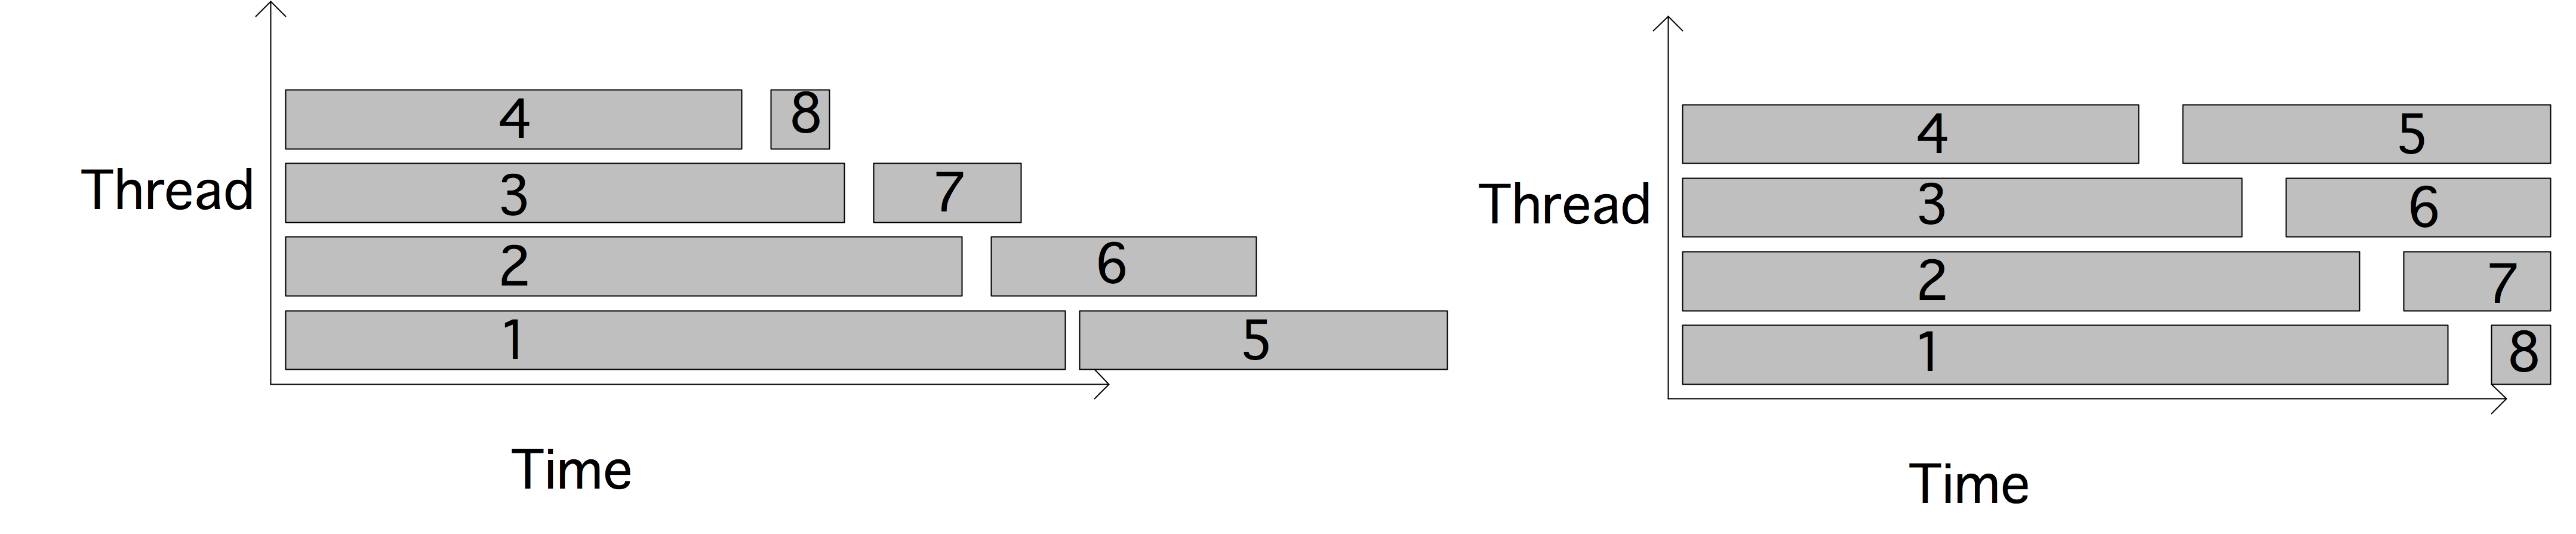
\includegraphics[scale=.07]{scheduling}
\end{frame}

\begin{frame}[containsverbatim]{Chunk size}
\small
  With $N$ iterations and $t$ threads:
  \begin{itemize}
  \item Static: each thread gets $N/t$ iterations.\\
    explicit chunk size: \texttt{schedule(static,123)}
  \item Dynamic: each thread gets $1$ iteration at a time\\
    explicit chunk size: \texttt{schedule(dynamic,45)}\\
  \item Help from OpenMP:\\
    guided schedule uses decreasing chunk size (with optional minimum
    chunk):\\
    \texttt{schedule(guided,6)}
  \end{itemize}
  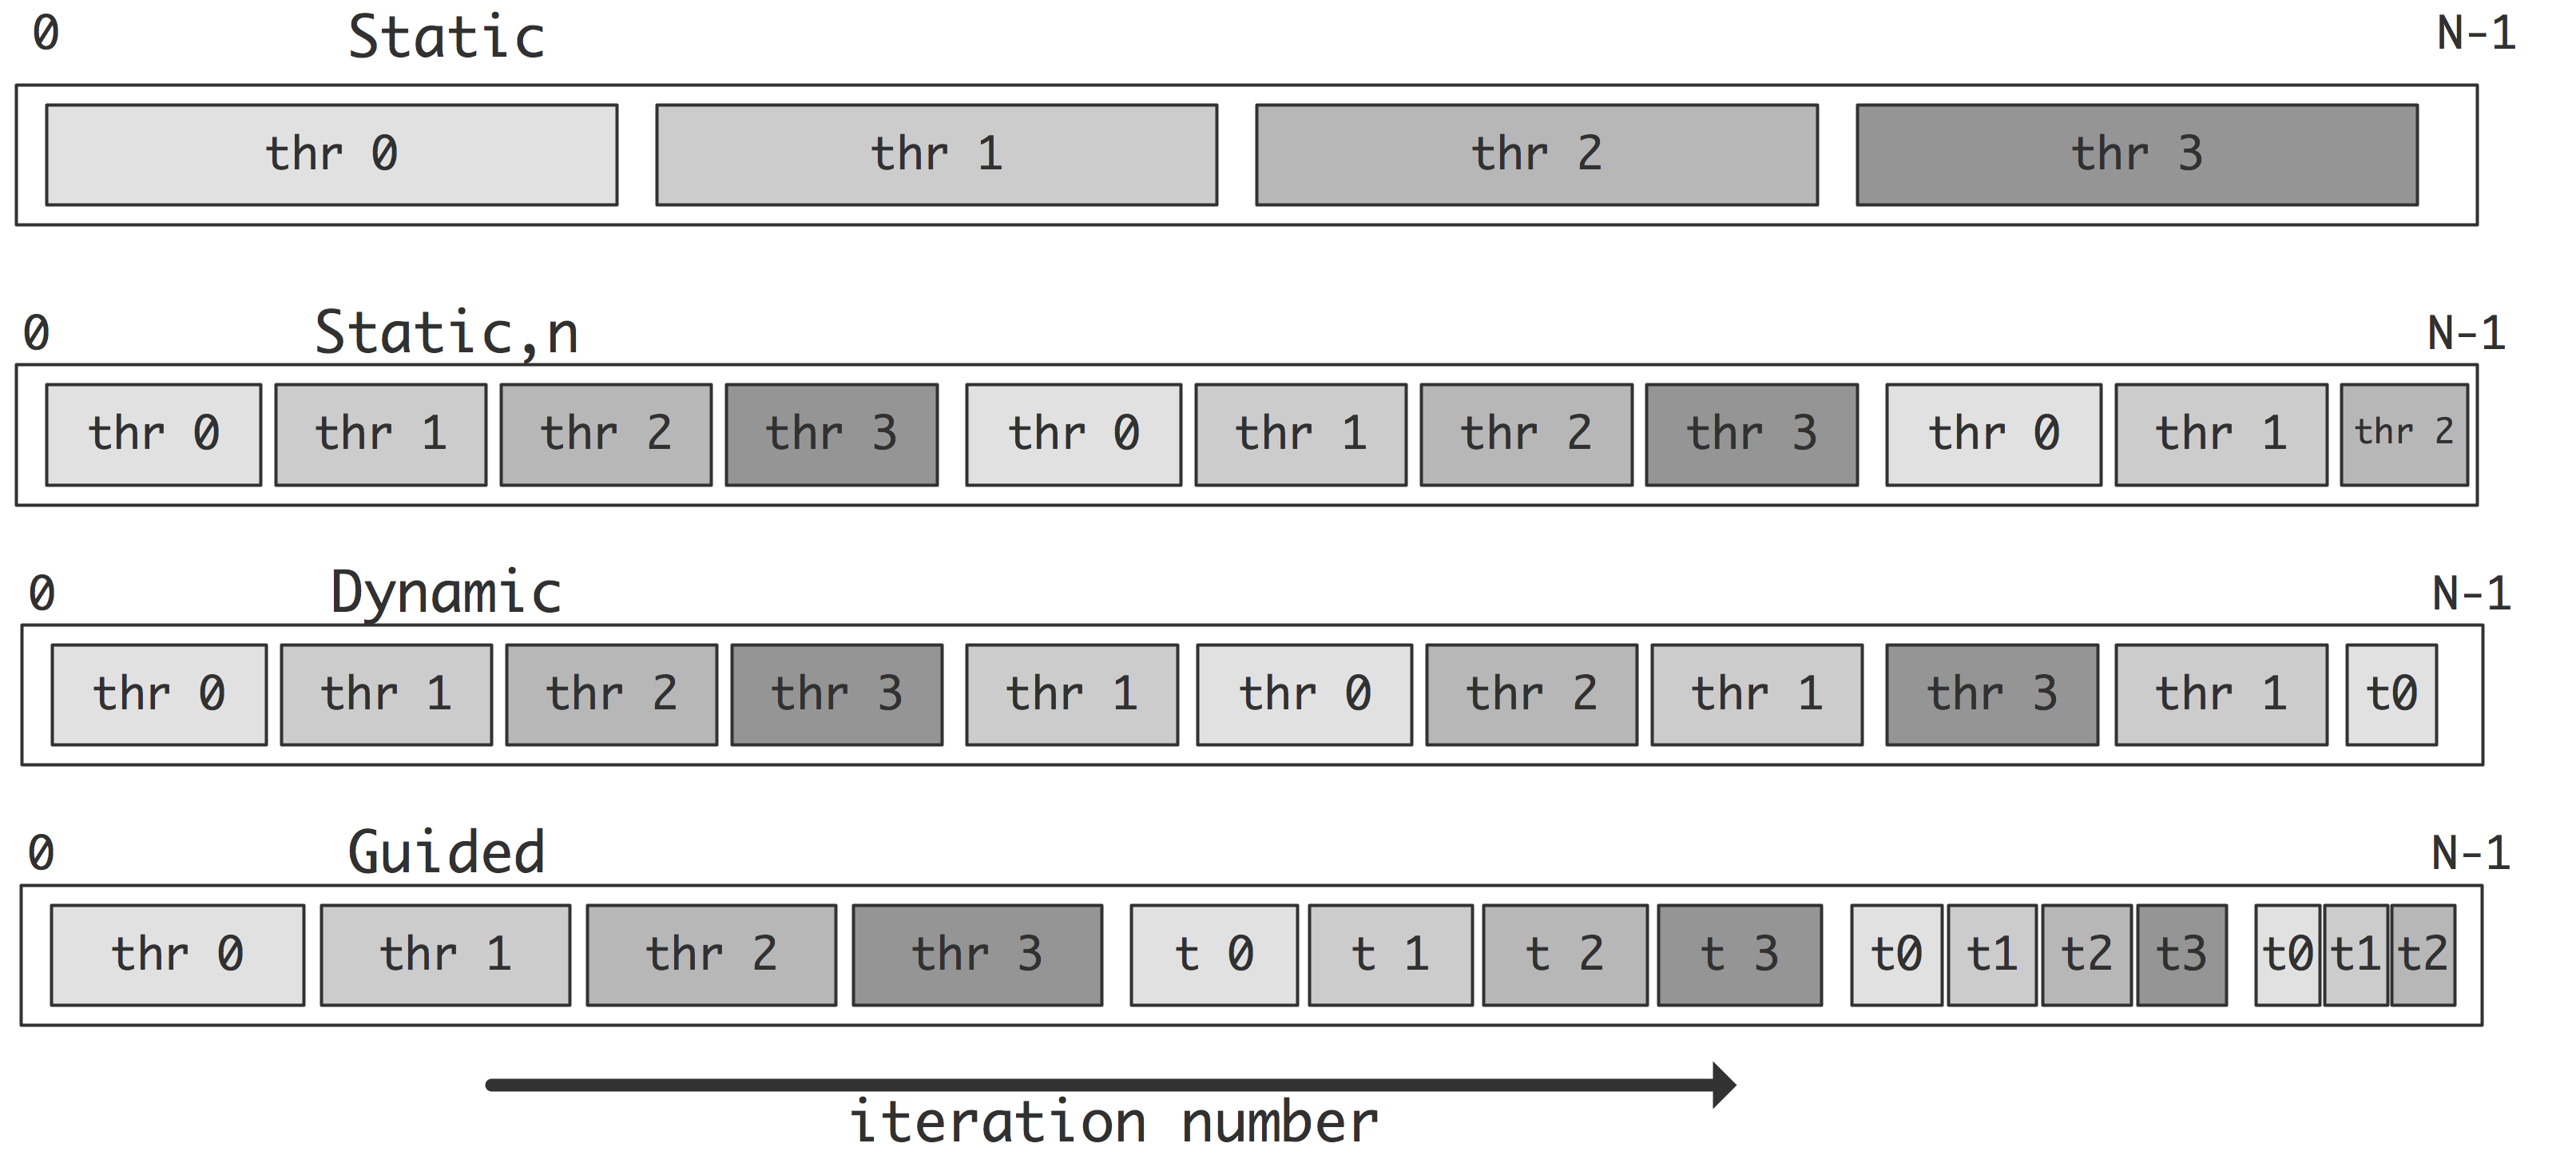
\includegraphics[scale=.08]{schedules}
\end{frame}

\begin{frame}[containsverbatim]{Reductions}
  \begin{itemize}
  \item Inner product loop:
\begin{verbatim}
s = 0.;
for (i=0; i<N; i++)
  s += x[i]*y[i];
\end{verbatim}
\item Use the \indextermtt{reduction(+:s)} clause.
  \item All the usual operations are available; you can also make your own.
  \end{itemize}
\end{frame}

\begin{exerciseframe}[piadapt]
  \footnotesize
  \input ex:omp-pi-adapt
\end{exerciseframe}

\begin{frame}[containsverbatim]{same exercise}
  \begin{enumerate}
  \item Use the \indextermtt{omp parallel for} construct to parallelize the loop.
    As in the previous lab, you may at first see an incorrect result.
    Use the \indextermtt{reduction} clause to fix this.
  \item Your code should now see a decent speedup, using up to 8~cores.
    However, it is possible to get completely linear speedup. For this
    you need to adjust the schedule.

    Start by using \indextermtt{schedule(static,$n$)}. Experiment with values
    for~$n$.  When can you get a better speedup? Explain this.
  \item Since this code is somewhat dynamic, try \indextermtt{schedule(dynamic)}.
    This will actually give a fairly bad result. Why?  Use
    \indextermtt{schedule(dynamic,$n$)} instead, and experiment with values
    for~$n$.
  \item Finally, use \indextermtt{schedule(guided)}, where OpenMP uses a
    heuristic.  What results does that give?
  \item \indextermtt{schedule(auto)} : leave it up to the system.
  \item \indextermtt{schedule(runtime)} : leave it up to environment variables;
    good for experimenting.
  \end{enumerate}
\end{frame}

\begin{frame}[containsverbatim]{More loop topics}
  \begin{itemize}
  \item Multiple loops can be collapsed: \indextermtt{collapse(2)}. Improves
    performance.
  \item Ordered iterations: normally OpenMP can execute iterations in
    any sequence. You can force ordering if you absolutely have
    to. Bad for performance!
  \item There is a barrier at the end of a \indextermtt{for}: use \indextermtt{nowait} to
    let threads continue.
  \end{itemize}
\end{frame}

\endinput

\begin{frame}[containsverbatim]{}
  \begin{itemize}
  \item 
  \end{itemize}
\end{frame}

